\documentclass{beamer}
\usepackage{fontspec}
\usepackage{xeCJK}
\setCJKmainfont{Noto Sans CJK SC}
\newfontfamily\Libertine[Mapping=tex-text]{Linux Libertine O}
\usetheme{Madrid}
\usecolortheme{crane}
\usepackage{polyglossia}
\setdefaultlanguage{english}
\setotherlanguage{thai}

\newfontfamily\thaifont[Script=Thai]{Noto Sans Thai}
\newfontfamily\thaifontsf[Script=Thai]{Noto Sans Thai}

\usepackage[e,f,j,k]{mtg2e}
\usepackage{xcolor}
\newcommand{\mtplain}[1]{\textcolor{teal}{#1}}
\renewcommand{\mtcitestyle}[1]{\mtplain{\textit{#1}}}
\newcommand{\tha}[1]{\mtplain{\textthai{#1}}}
\newcommand{\zh}[1]{\mtplain{#1}}
\newcommand{\msa}{\mtciteform}

% Set the Thai font for Thai language text
%\setotherlanguage{thai}
%\newfontfamily\thaifamily{Noto Sans Thai}[Script=Thai]

\usepackage{mygb4e}
\renewcommand{\eachwordtwo}{\Libertine}

\title{Languages of South East Asia and China}
\author[Francis Bond]{Francis Bond \\ based on slides by František Kratochvíl}
\date{2024}\begin{document}

\frame{\titlepage}

\begin{frame}{Overview}

\begin{itemize}
\item  Recognised language families of the region
\item Impact of geography on human population movement, linguistic diversity
and cultures of MSEA
\item Indospheric and Sinospheric influences

\item Typological features of MSEA languages
\begin{itemize}
\item Lexical tone
\item Phoneme inventories
\item Zero anaphora
\item Classifier systems
\item Serial verb constructions
\end{itemize}
\item What makes MSEA a linguistic area, and why?
\end{itemize}
\end{frame}

\begin{frame}{Official Languages}
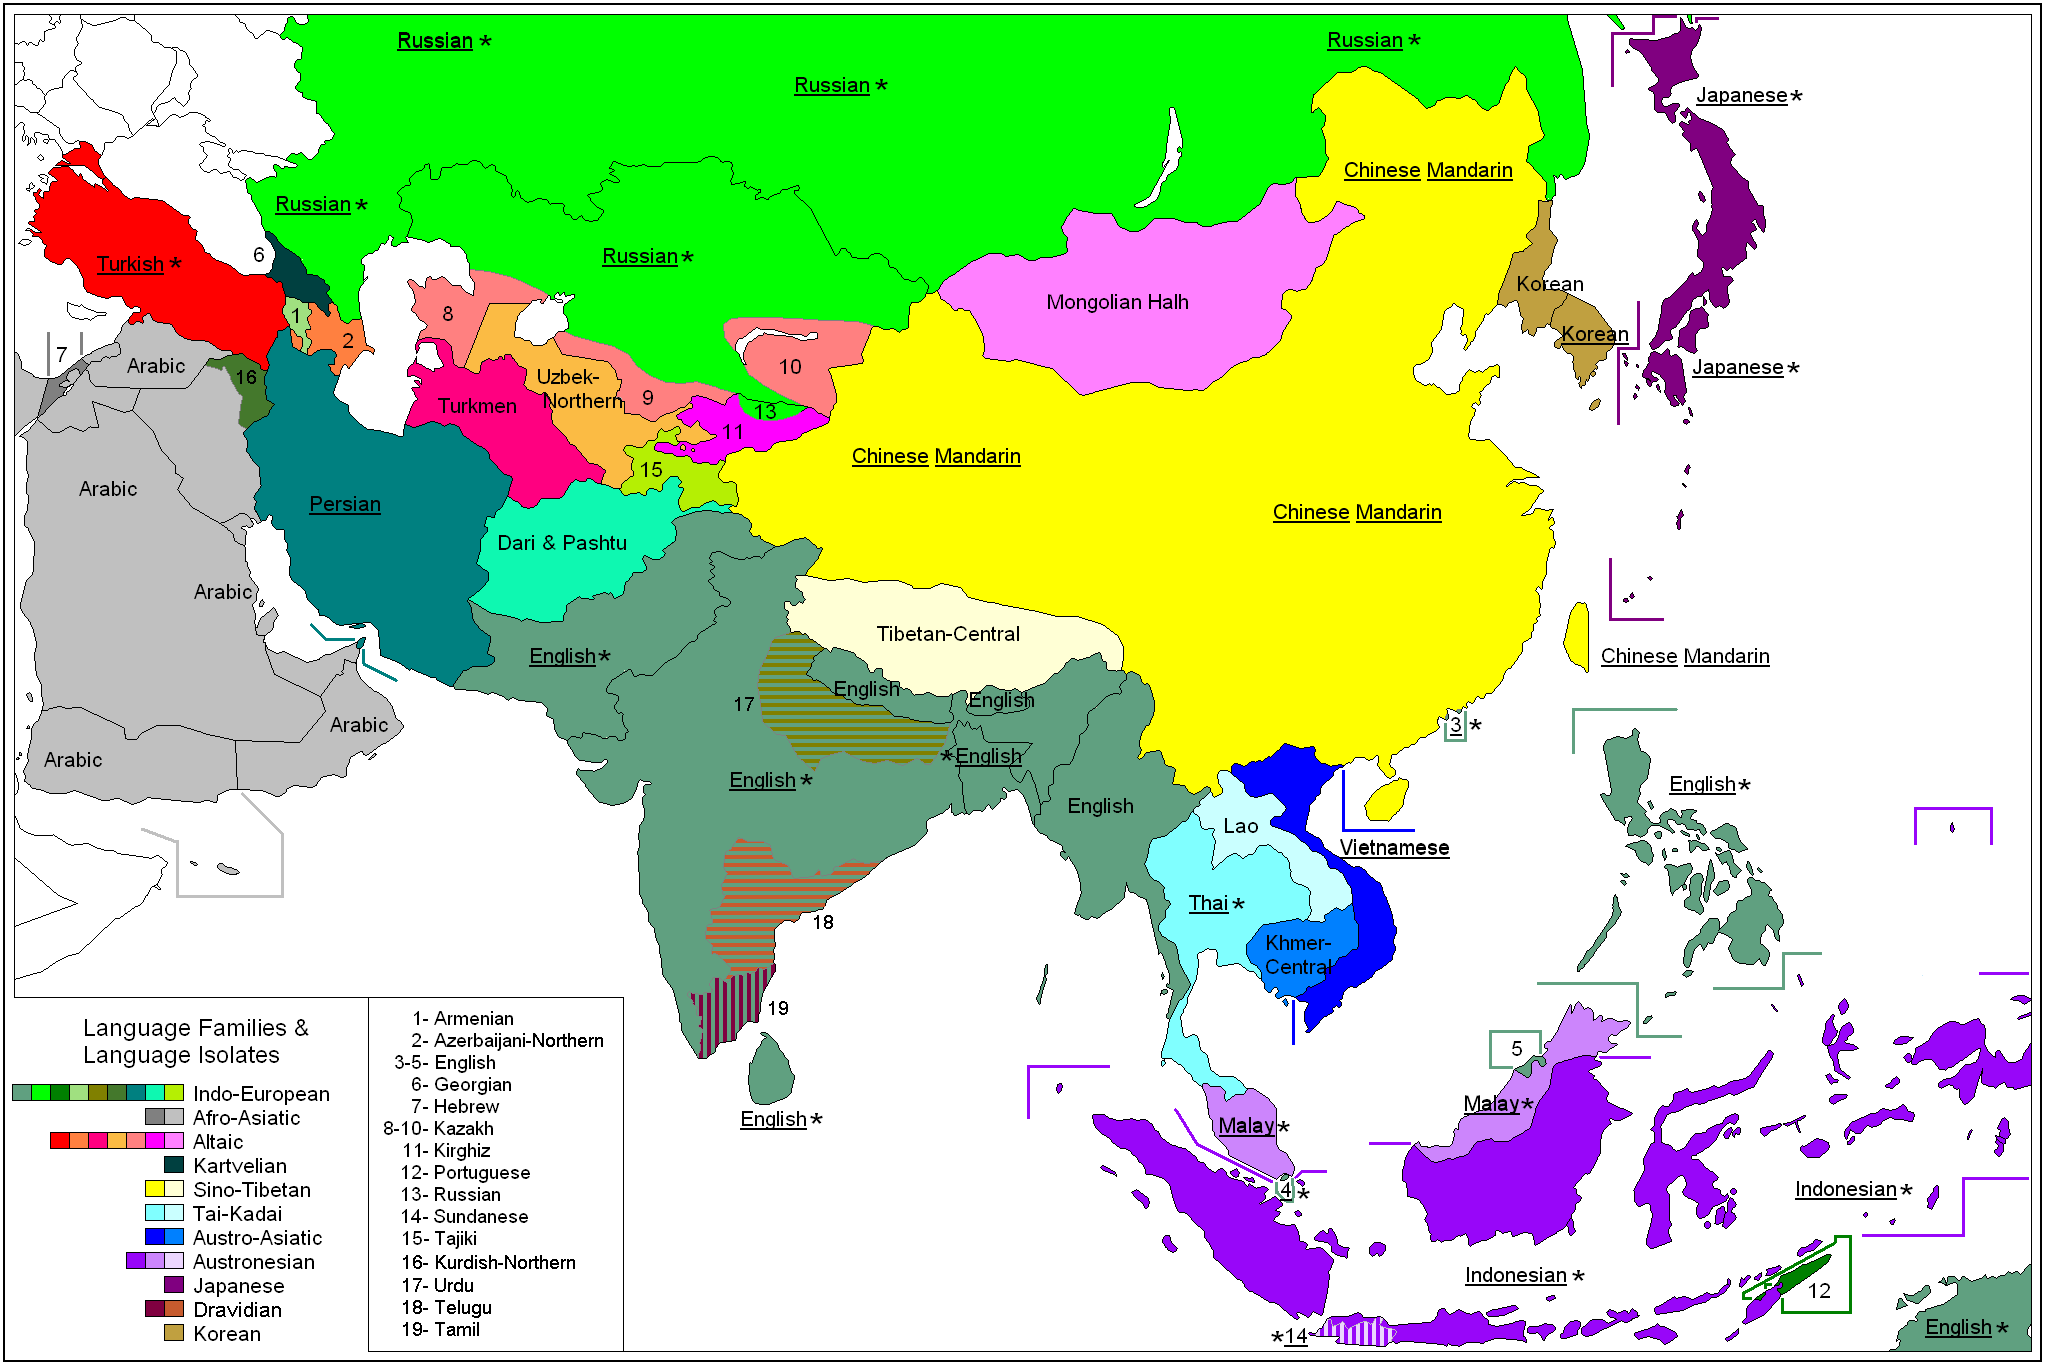
\includegraphics[width=\textwidth]{pics/image1.png}
\end{frame}


\begin{frame}{The major language families of SEA}
  \begin{itemize}

\item \textbf{Austronesian}: mainly in coastal regions of Vietnam, Burma and
western peninsular SEA.

\item \textbf{Austroasiatic} (Mon-Khmer branch -- Munda branch is only found
in South Asia): widely scattered throughout MSEA region and extending
into NE India (Khasian branch).

\item \textbf{Sino-Tibetan}
\begin{itemize}
\item \textbf{Tibeto-Burman} Burma, NE India,
mountainous regions of Western and northern Thailand, Laos and northern
Vietnam.
\item \textbf{Sinitic}  predominantly China
\end{itemize}

\item \textbf{Tai-Kadai}: southern China, SEA, NE India.

\item \textbf{Hmong-Mien}: (a.k.a. Miao-Yao): mostly in southern China,
extending into SEA.
\item \textbf{Korean, Japanese and Ainu}: Korean Peninsular and Japan
\end{itemize}  
MSEA forms a linguistic area in which many languages share similar
features despite being geneDcally unrelated.

\end{frame}

\begin{frame}{The countries/regions of MSEA}

  \begin{tabular}{cc}

    \begin{minipage}[b]{0.45\textwidth}\raggedright
      \begin{itemize}
      \item Burma
      \item Cambodia
      \item Laos
      \item Malaysia
      \item Thailand
      \item Vietnam
      \item NE India (arguably eastward of the
        south bank of the Brahmaputra River)
      \end{itemize}
\end{minipage} &
                 \begin{minipage}[b]{0.45\textwidth}
 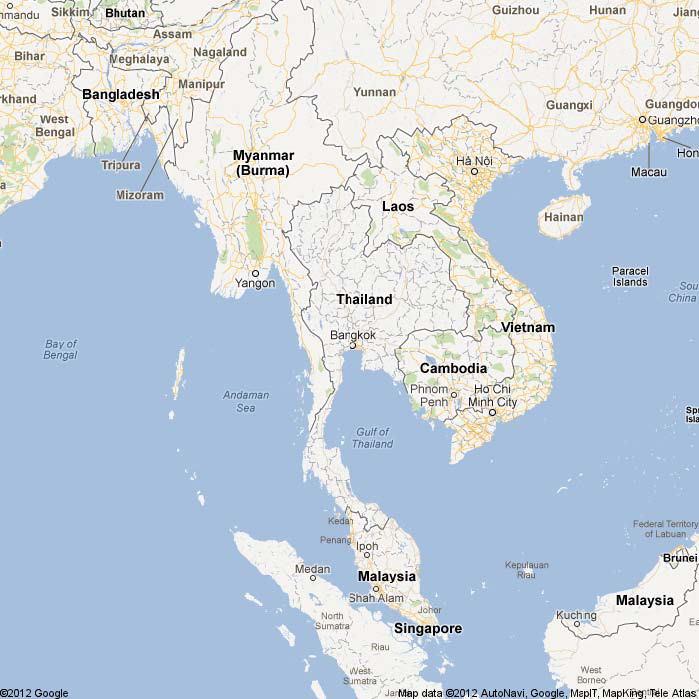
\includegraphics[width=\textwidth]{pics/image2.png}
 \end{minipage} 
  \end{tabular}

  \medskip

  Much of Mainland Southeast Asia is very mountainous.  The people of the uplands have long resisted  being governed by central states of the lowland basins.
%\citep{Scott:2009}
%   James ScoZ's\\
% 2009 book, \emph{The Art of Not Being Governed: An Anarchist History of
% Upland Southeast Asia}, discusses the strategies that the people of this
% region -- which he refers to as ``Zomia'' -- have employed to\\
% avoid being governed by central states of the lowland basins.

  
\end{frame}


\begin{frame}{Human and linguistic diversity in MSEA}
\begin{itemize}

\item Mainland Southeast Asia (MSEA) is recognised for its high degree of
human diversity in comparison to the global average.

\item This refers to diversity in all measures of distinction among human groups, including social structure, material culture, and genetic markers.

\item The diversity of languages, however, has been regarded as relatively
low, although they number around 2000. Why?
\end{itemize}

\end{frame}

\begin{frame}
  \begin{itemize}
    \item \textbf{Language Families}: Many languages in MSEA belong to a small number of language families (Austroasiatic, Tai-Kadai, Sino-Tibetan, Hmong-Mien), leading to similarities that reduce the perception of diversity.
    \item \textbf{Contact and Convergence}: Long history of contact, trade, migration, and cultural exchange has led to linguistic convergence, creating similar features across unrelated languages.
    \item \textbf{Multilingualism and Language Shift}: High rates of multilingualism and the use of lingua francas (e.g., Thai, Vietnamese) often overshadow smaller languages, making linguistic diversity less visible.
    \item \textbf{Linguistic Classification}: Differences in how linguists classify languages and dialects can influence the perceived number of languages, sometimes reducing the apparent diversity.
\end{itemize}
\end{frame}


\begin{frame}{Austroasiatic}
The Austroasiatic family (AA) forms two major 
branches: \textbf{Munda}, spoken only in India, and \textbf{Mon-Khmer}, constituting more than 120 languages spoken in an area
extending from Meghalaya state in NE India to Vietnam in the east, and
the Malay peninsula in the south.

AA languages are also spoken in China.
\end{frame}

\begin{frame}
  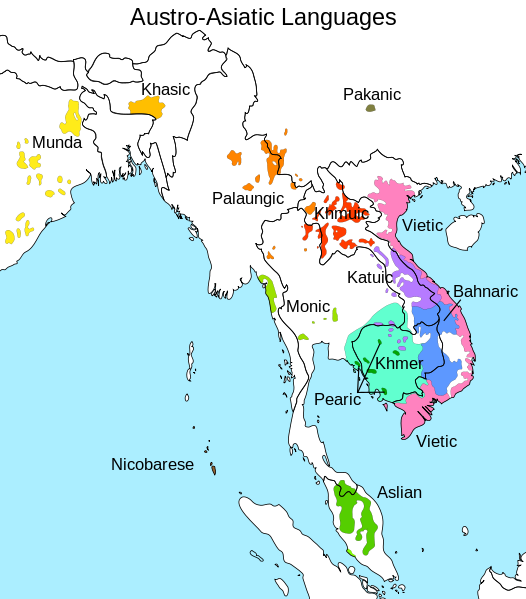
\includegraphics[width=0.9\textwidth]{pics/image5.png}
\end{frame}





\begin{frame}{Austronesian}

Austronesian is the largest and most widespread family in the
world, with somewhere around 700 (maybe as many as 1,200) languages
altogether and 300 million native speakers. Aside from Southeast Asia,
Austronesian languages are found on numerous islands in the eastern and
central Pacific Ocean all the way to Easter Island. There is also a western
outpost language (Malagasy), spoken on the island of Madagascar.

Major languages include:
\begin{itemize}
\item Malay (200 million speakers, about 40 million as a first language)
  \\  Indonesian (Bahasa Indonesia) and Malaysian (Bahasa Melayu)
\item Javanese (75 million)
\item Sundanese (30 million)
\item Pilipino (Tagalog) (50 million, 17 million as a first language).
\end{itemize}
  
\end{frame}

\begin{frame}
  
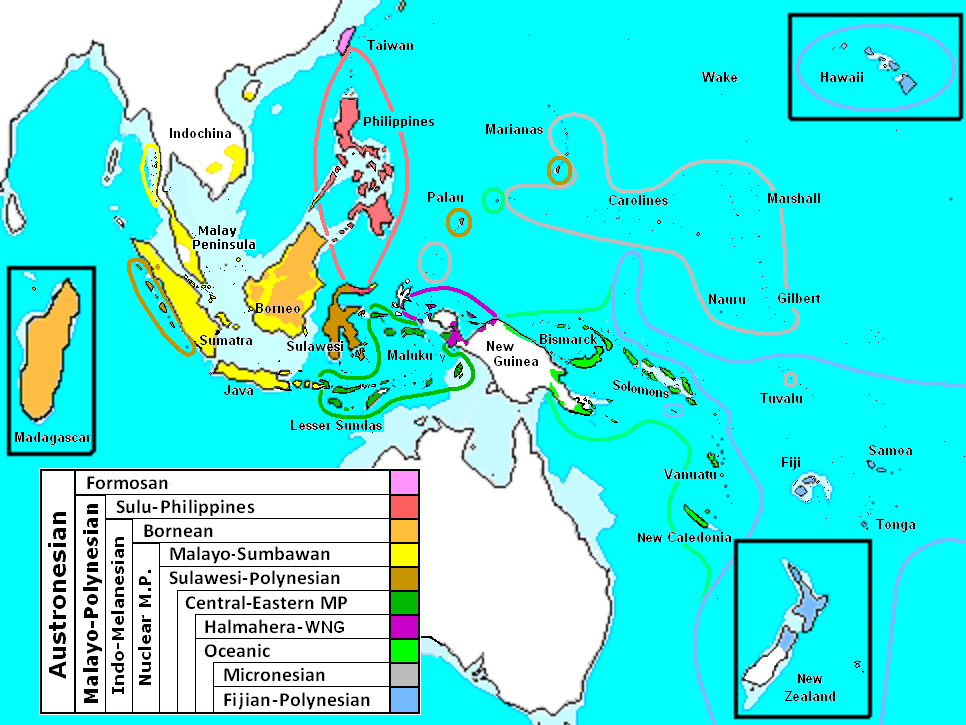
\includegraphics[width=0.9\textwidth]{pics/image4.png}
\end{frame}

\begin{frame}{Mon-Khmer branch of Austroasiatic}
\begin{itemize}
\item  Aslian (mostly endangered), spoken in southern Thailand and Western
Malaysia.

\item Katuic-Bahnaric, spoken in Vietnam, Laos, NE Thailand and Cambodia.

\item Northern Mon-Khmer, which divides into Palaungic and Khumic, spoken in
Yunnan and adjacent areas of Burma, Northern Thailand, and NE Laos.

\item Vietic languages, spoken in Vietnam (including Vietnamese)

\item Monic, spoken by increasingly diminishing numbers of speakers in Burma
and Central Thailand.

\item Pearic, spoken by small groups in Western Cambodia and adjacent areas
of NE Thailand.

\item A Pakanic branch has recently been proposed for a group of languages
spoken in northern Vietnam, and in Guanxi and Yunnan, China.

\end{itemize}
  
There are many competing classifications of the Mon-Khmer branch in the
literature, none of which has received universal acceptance.
\end{frame}

\begin{frame}{Major Mon-Khmer languages}
\begin{itemize}
\item Khmer (Cambodian, about 13 million speakers)
\item Vietnamese (nearly 70 million)
\end{itemize}

\begin{center}
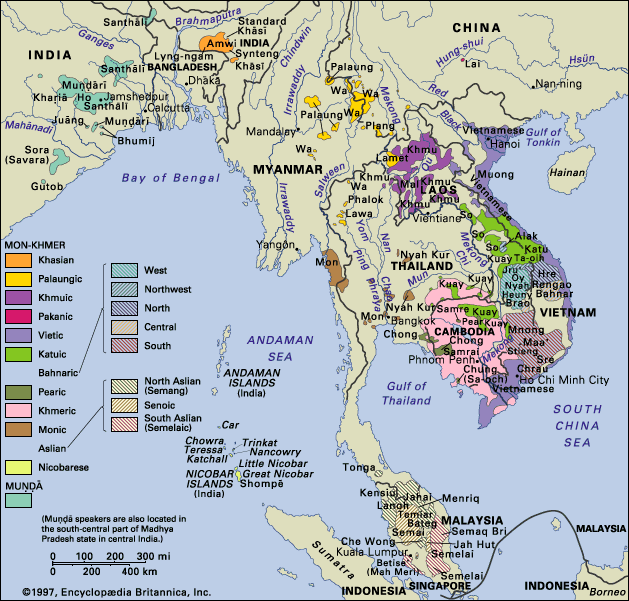
\includegraphics[height=.7\textheight]{pics/image6.png}
\end{center}
\end{frame}

\begin{frame}{Tibeto-Burman}

Most of the roughly 300 Tibeto-Burman languages are found in the South Asian
region, but many of them straddle the buffer zone between South Asia and
Southeast Asia.

Overall, the Tibeto-Burman languages can be quite different from Sinitic
languages, with agglutinative morphology, verb final word order, and postpositions.

Major languages:

\begin{itemize}
\item Burmese (30 million speakers)
\item Tibetan (5 million)
\item Karen  (4 million combined: S'gaw is
the largest, at about 2 million)
\item Lolo (Yi) (3 million, spoken in China)
\item Bai (1 million, spoken in China).
\end{itemize}

  
\end{frame}

\begin{frame}
  \begin{center}
  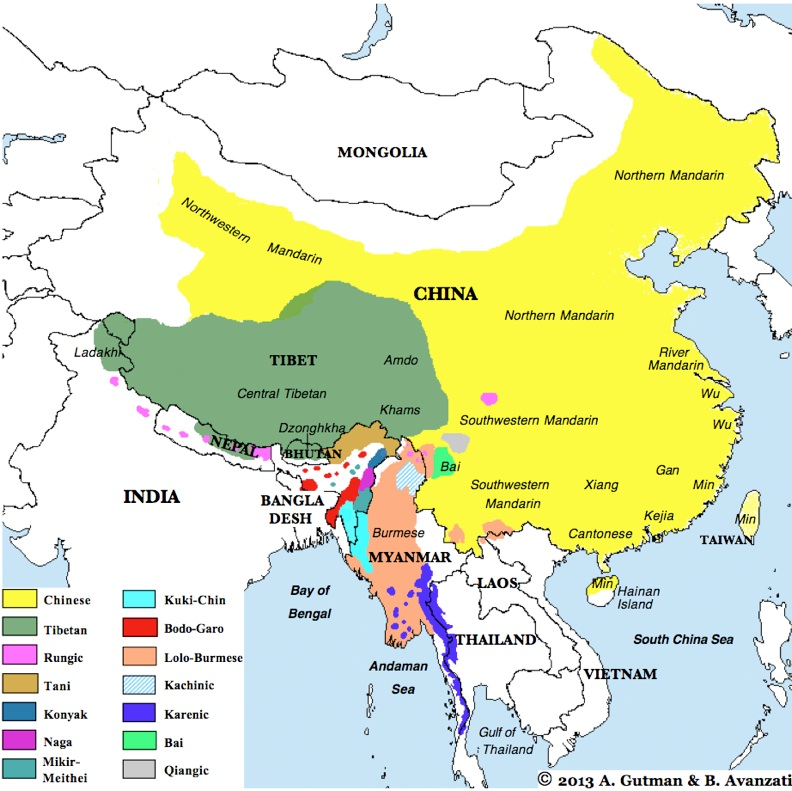
\includegraphics[height=0.9\textheight]{pics/tibeto-burman-map}
\end{center}
\end{frame}

\begin{frame}{Sinitic Languages}

Sinitic languages are spoken by a huge number of people (over 1,000 million)
in mainland China, and Taiwan, and in Southeast Asia.
\begin{itemize}
\item Mandarin
  \begin{itemize}
  \item Northern
  \item Jiang-Huai/Southeastern (Jiangsu and Anhui)
  \item Southwest (Hubei, Sichuan, Yunnan, Guizhou, eastern Hunan, western Guangxi)
  \end{itemize}
\item Wu (Southern Jiangsu, Zhejiang)
\item Xiang (Hunan)
\item Yue (Guangdong, Guangxi, parts of Hainan)  Cantonese
\item Min (Fujian, Taiwan, parts of Hainan)  Hokkien
\item Gan (Jiangxi, north-eastern Guangdong)
\item Hakka (southern Jiangxi, north-eastern Guangdong, western Fujian, part
of Sichuan, Guangxi, and Taiwan)
\end{itemize}

\end{frame}

\begin{frame}{Major Chinese Dialect Groups and Number of Speakers}
  \begin{center}
\begin{tabular}{lc}
\hline
\textbf{Dialect Group} & \textbf{Number of Speakers (millions)} \\ \hline
Mandarin & 900+ \\ \hline
Wu (e.g., Shanghainese) & 80+ \\ \hline
Xiang (Hunanese) & 36+ \\ \hline
Yue (Cantonese) & 85+ \\ \hline
Min (e.g., Hokkien, Teochew) & 70+ \\ \hline
Gan & 22+ \\ \hline
Hakka & 45+ \\ \hline
\end{tabular}

\end{center}

The numbers are approximate and can vary due to factors such as migration and classification. 
\end{frame}

\begin{frame}
  According to Goddard (p55)
  \begin{quote}
    As mentioned earlier, in the Chinese tradition any variety other
than Mandarin is referred to as a ``dialect''. This practice reflects the cultural
and historical unity of China and the use of a common script, but it is con-
fusing because in linguistic usage the term dialect implies mutual intel-
ligibility. Linguists usually refer to the seven language groupings just
mentioned as ``Sinitic languages'', and that is what we will do in this book too;
but it is not entirely satisfactory, because some of these ``languages'' have
many mutually unintelligible varieties. For example, Min is reported to
have nine mutually unintelligible varieties in the Fujian province alone
(Li 1992). On strictly linguistic criteria there are probably hundreds of Sinitic
languages in China (which is not surprising, really, in view of the population
size).
  \end{quote}
\end{frame}


\begin{frame}
  \begin{center} 
    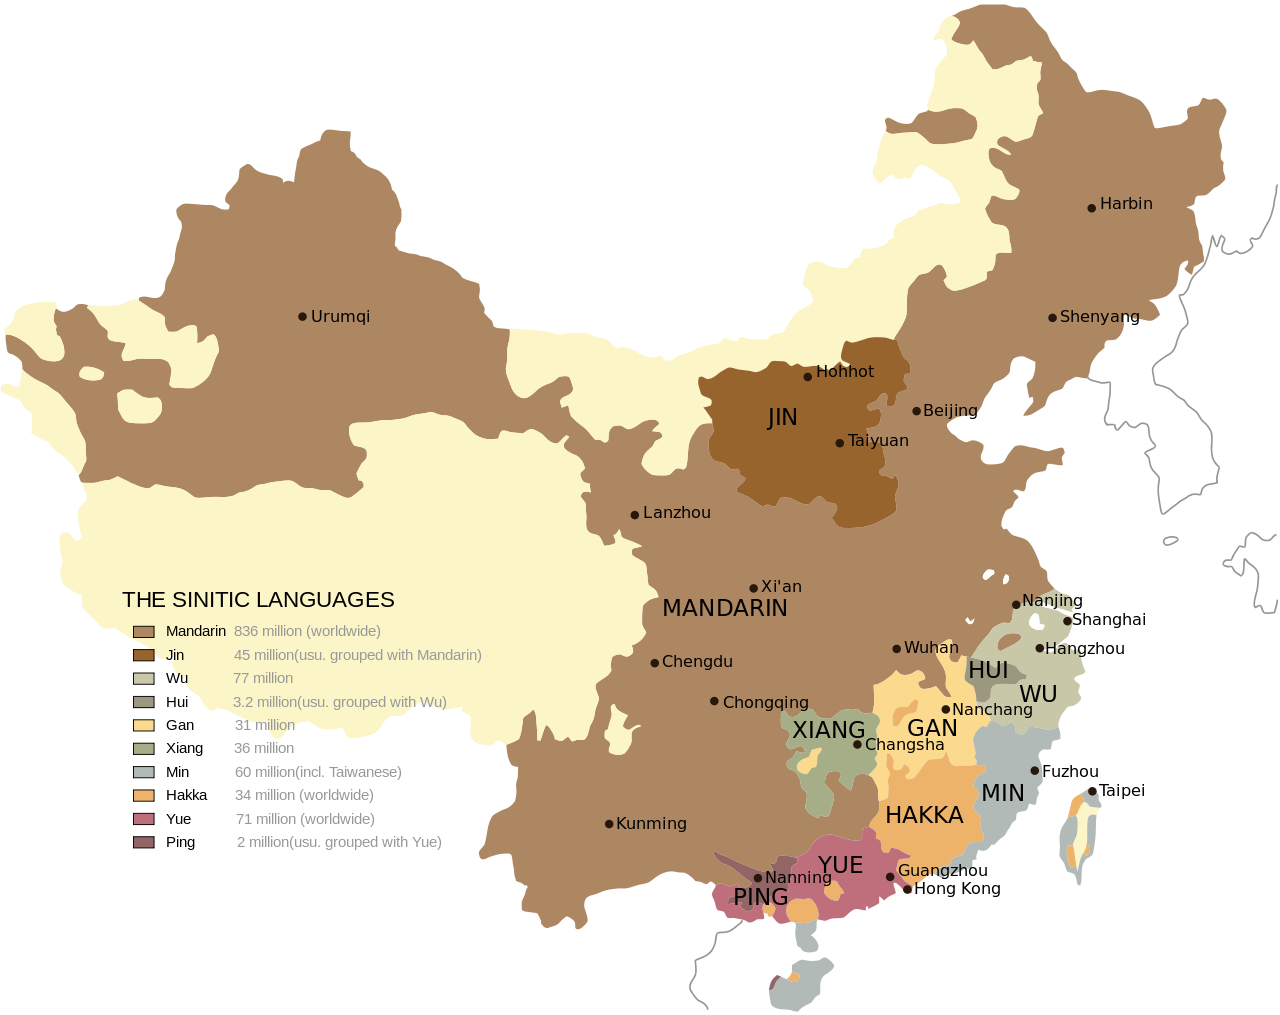
\includegraphics[height=0.9\textheight]{pics/image15.png}
  \end{center}
\end{frame}



\begin{frame}

Return the money to me
\begin{exe}

\ex
\glll 把 钱 还 给 我 \\
     pa³²⁴ tɕʰjæn²⁵ xwan²⁵ kej³²⁴ wɔ³²⁴ \\
     take money return give 1\textsc{sg} \\ 
  \hfill     \textit{Mandarin (Putonghua)}
     
\ex \glll  畀 返 D 钱 我 \\
 pei³⁵ fæ:n⁵⁵ ti⁵⁵ tɕʰin³⁵ ŋɔ¹³ \\
 give back \textsc{pl.cl} money 1\textsc{sg} back \\
\hfill  \textit{Yue (Hong Kong)}

\ex \glll 铜钱 还 给 我 \\
      doŋ²²-dʑi⁵⁵ wæj³⁵ paʔ⁵ niʔ⁵ \\
     money return give 1\textsc{sg} \\
 \hfill  \textit{Wu dialect (Suzhou)}


\ex \glll 钱 倒 还 与 我 \\
  tɕı̃³⁵ tɔ⁵⁵ huan³⁵ ho²² gua⁵³ \\
 money invert return give 1\textsc{sg} \\
 \hfill \textit{Southern Min (Quanzhou)}
  
\end{exe}
 
\end{frame}


\begin{frame}{Mandarin Romanization Comparison}
  \begin{tabular}{llll}\small

Characters & Wade-Giles & Hanyu Pinyin & Notes\\ \hline
中国/中國 & Chung¹-kuo² & Zhōngguó & China\\ 
北京 & Pei³-ching¹ & Běijīng & PRC Capital \\
    台北 & T'ai²-pei³ & Táiběi & RoC Capital \\
                                 
毛泽东/毛澤東 & Mao² Tse²-tung¹ & Máo Zédōng & Mao \\
蒋介石/蔣介石 & Chiang³ Chieh⁴-shih² & Jiǎng Jièshí & Chiang Kai-shek \\
孔子 & K'ung³ Tsu³ & Kǒng Zǐ & Confucius \\ 
  \end{tabular}
  \bigskip
  
  There is also a native  transliteration system for Standard Chinese and other Sinitic languages: \textbf{Bopomofo}. It is commonly used in Taiwan. It consists of 37 characters and five tone marks, which together can transcribe all possible sounds in Mandarin Chinese:  ㄓㄨㄥ ㄍㄨㄛˊ , ㄅㄟˇ ㄐㄧㄥ, ㄊㄞˊ ㄅㄟˇ , ㄇㄠˊ ㄗㄜˊ ㄉㄨㄥ,  ㄐㄧㄤˇ ㄐㄧㄝˋ ㄕˊ, ㄎㄨㄥˇ ㄗˇ

  
  
% \textbf{Characters} & \textbf{Wade-Giles} & \textbf{Hanyu Pinyin} & \textbf{Bopomofo} \\ \hline
% 中国/中國 & Chung¹-kuo² & Zhōngguó & ㄓㄨㄥ ㄍㄨㄛˊ \\ \hline
% 北京 & Pei³-ching¹ & Běijīng & ㄅㄟˇ ㄐㄧㄥ \\ \hline
% 台北 & T'ai²-pei³ & Táiběi & ㄊㄞˊ ㄅㄟˇ \\ \hline
% 毛泽东/毛澤東 & Mao² Tse²-tung¹ & Máo Zédōng & ㄇㄠˊ ㄗㄜˊ ㄉㄨㄥ \\ \hline
% 蒋介石/蔣介石 & Chiang³ Chieh⁴-shih² & Jiǎng Jièshí & ㄐㄧㄤˇ ㄐㄧㄝˋ ㄕˊ \\ \hline
% 孔子 & K'ung³ Tsu³ & Kǒng Zǐ & ㄎㄨㄥˇ ㄗˇ \\ \hline
% \end{tabular}
\end{frame}

\begin{frame}{Sinospheric features}

Sino-Tibetan languages found in SEA are more likely to have features in
common with Sinitic languages -- e.g.

\begin{itemize}
\item complex tone
\item classifiers
\item limited morphology
\item isolating word formation
\item pragmatically determined syntax
\item reliance on zero anaphora
\end{itemize}
\end{frame}

\begin{frame}{Indospheric features}


Sino-Tibetan languages found in South Asia are more likely to have
features in common with Indic languages, e.g.

\begin{itemize}
\item simple tone systems or no lexical tone
\item morphologically complex stems
\item fusional or agglutinative word formation
\item breathy and retroflex consonants
\item pronominal cross-referencing on the verb
\item well-developed case-marking paradigms
\end{itemize}
\end{frame}

\begin{frame}{Tai-Kadai}

The Tai-Kadai (onen simply Tai) family splits into three branches:
  \begin{itemize}
\item Northern

\item Central

\item South-western
\end{itemize}

Thai is a member of the South-western branch, members of which can be
found as far west as Assam in NE India.

The established spelling convention is that `Tai' (pronounced with an
unaspirated dental stop \emph{t}) is used for the family name, and
`Thai' (pronounced with an aspirated dental stop \emph{th}) is
normally used to refer to the national language of Thailand.

\end{frame}

\begin{frame}
  \begin{center}
  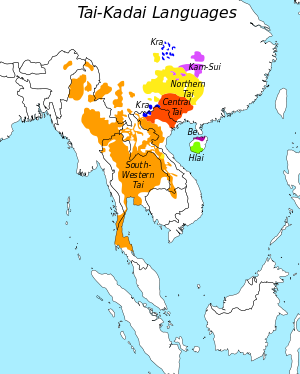
\includegraphics[height=0.9\textheight]{pics/image27.png}
\end{center}
\end{frame}


\begin{frame}{Historical origin of Tai-Kadai languages}


Tai-Kadai languages are descended from a parent language estimated to
have been spoken by a single group of people approximately fineen
hundred to two thousand years ago.

Most linguists think that the Tai homeland was somewhere near the
present-day Vietnam/China border. Tai speakers are believed to have migrated from this region to northern
Vietnam

  \begin{itemize}
\item Laos
\item Thailand
\item southern provinces of China

\item northern Burma
\item Assam in north-eastern India
\end{itemize}
\end{frame}


\begin{frame}{Major Tai-Kadai Languages}
  \begin{itemize}
  \item Thai (60 million speakers)
    \\ could be several languages
  \item Lao (4 million)
  \end{itemize}

Over 50 other Tai-Kadai languages.
\end{frame}

\begin{frame}{Hmong-Mien}

  Thirty-five languages spoken mainly in southwestern
  China, with several spoken in adjacent parts of Southeast Asia.

  \begin{itemize}
  \item Hmong (also known as Miao: 5 million speakers)
  \item Mien (also known as Man and as Yao: 2 million)
  \end{itemize}

Most work has been done on this family by Chinese scholars, and it is
relatively little known in the West.   It is mainly spoken in the hills.
  
\end{frame}


\begin{frame}
  \begin{center}
    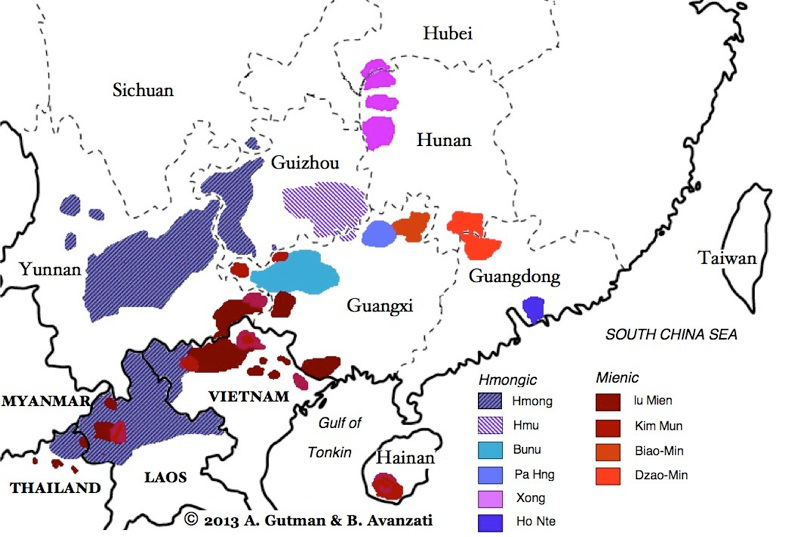
\includegraphics[height=0.9\textheight]{pics/image8.png}
  \end{center}
\end{frame}

\begin{frame}{Japanese, Korean, and Ainu}
  \begin{itemize}
  \item Japanese (125 million speakers)
  \item Korean (70 million)
  \item Ainu (isolate, fewer than 300 speakers) 
  \end{itemize}

Japanese and Korean share very similar syntax (agglutinative, case marking, verb final, pre-modification) and both have borrowed much vocabulary from Chinese.
  
\end{frame}
\begin{frame}
  \begin{center}
    \huge Mainland Southeast Asia as a Linguistic Area
  \end{center}
\end{frame}

\begin{frame}{Mainland Southeast Asia as a Linguistic Area}
    \begin{itemize}
        \item Languages of different families often converge when in close contact.
        \item A "linguistic area" (\textit{Sprachbund}) is where unrelated languages share features.
        \item Mainland Southeast Asia is a linguistic area due to long mutual influence.
        \item Shared features span phonology, lexicon, and grammar.
        \item Example: Limited syllable structures and presence of lexical tone.
        \item Many features shared with non-mainland languages
    \end{itemize}
\end{frame}


% Slide 2
\begin{frame}{Shared Phonological Features}
    \begin{itemize}
        \item Many languages have a limited range of syllable structures.
        \item Lexical tone is common across the region.
        \item Example: Tones in Vietnamese, Thai, and many Chinese dialects.
        \item Mon-Khmer languages often lack tones, with some exceptions.
        \item Phonological convergence results from prolonged contact.
    \end{itemize}
\end{frame}


\begin{frame}[allowframebreaks]{Phonological Features: Examples}
    \begin{itemize}
        \item \textbf{Limited syllable structures}:
            \begin{itemize}
                \item \textbf{Mandarin Chinese} primarily uses simple syllables like CV (Consonant-Vowel) and CVN (Consonant-Vowel-Nasal), e.g.,
                    \begin{itemize}
                        \item \textit{mā} (mother)
                        \item \textit{màn} (slow)
                    \end{itemize}
                \item Complex consonant clusters are rare in these languages.
            \end{itemize}
        \item \textbf{Lexical tone examples}:
            \begin{itemize}
                \item \textbf{Mandarin Chinese} has four tones:
                    \begin{itemize}
                        \item \textit{mā} (mother) – high-level tone
                        \item \textit{má} (hemp) – rising tone
                        \item \textit{mǎ} (horse) – dipping tone
                        \item \textit{mà} (scold) – falling tone
                        \end{itemize}
                        \framebreak
                \item \textbf{Thai} has five tones:
                    \begin{itemize}
                        \item \textit{maa} (come) – mid tone
                        \item \textit{máa} (horse) – rising tone
                        \item \textit{màa} (dog) – low tone
                        \item \textit{mâa} (mother) – falling tone
                        \item \textit{măa} (new) – high tone
                    \end{itemize}
                \item \textbf{Vietnamese} has six tones, e.g.,
                    \begin{itemize}
                        \item \textit{ma} (ghost) – level tone
                        \item \textit{má} (cheek) – high rising tone
                        \item \textit{mà} (but) – low falling tone
                        \item \textit{mả} (tomb) – falling-rising tone
                        \item \textit{mã} (horse) – glottalized rising tone
                        \item \textit{mạ} (young rice plant) – glottalized falling tone
                    \end{itemize}
            \end{itemize}
    \end{itemize}
\end{frame}




% Slide 3
\begin{frame}{Shared Morphological Features}
    \begin{itemize}
        \item Lack of inflectional morphology is widespread.
        \item Use of classifier constructions is a common feature.
        \item Example: Classifiers used when counting nouns in Thai and Mandarin.
        \item Morphological similarities facilitate language learning across groups.
        \item Reflects a mutual adaptation over time.
    \end{itemize}
\end{frame}
\begin{frame}{Classifiers in Thai and Mandarin}
    \begin{itemize}
        \item \textbf{Mandarin Chinese} classifiers:
            \begin{itemize}
                \item \zh{一只猫} (yī zhī māo) – "one (zhī) cat"
                \item \zh{三本书} (sān běn shū) – "three (běn) books"
                \item \zh{五辆车} (wǔ liàng chē) – "five (liàng) cars"
            \end{itemize}
        \item \textbf{Thai} classifiers:
            \begin{itemize}
                \item \tha{เด็กหนึ่งคน} (dèk nùeng khon) – "one (khon) child"
                \item \tha{บ้านสองหลัง} (bâan sǎawng lǎng) – "two (lǎng) houses"
                \item \tha{เสื้อผ้าสามตัว} (sûea phâa sǎam tua) – "three (tua) shirts"
            \end{itemize}
        \item Classifiers are essential when quantifying nouns.
    \end{itemize}
  \end{frame}
  
% Slide 4
\begin{frame}{Areal Lexicon}
    \begin{itemize}
        \item Beyond shared words, languages share conceptual frameworks.
        \item Term "areal lexicon" coined by James Matisoff.
        \item Shared worldview and consensus on topics worth discussing.
        \item Example: Similar cultural vocabulary across unrelated languages.
        \item Reflects deep cultural and linguistic exchange.
    \end{itemize}
\end{frame}

\begin{frame}[allowframebreaks]{Areal Lexicon: Shared Cultural Vocabulary}
    \begin{itemize}
        \item \textbf{Shared terms for "rice" at different stages}:
            \begin{itemize}
                \item \textbf{Thai}:
                    \begin{itemize}
                        \item \textit{khao} (\tha{ข้าว}) – rice in general
                        \item \textit{khao niao} (\tha{ข้าวเหนียว}) – sticky rice
                    \end{itemize}
                  \item \textbf{Vietnamese}:
                    \begin{itemize}
                    \item \textit{lúa} – rice plant
                    \item \textit{gạo} – uncooked rice grains
                    \item \textit{cơm} – cooked rice
                    \end{itemize}
                  \item \textbf{Japanese}:
                    \begin{itemize}
                    \item \jpn{稲} \textit{ine} – rice plant
                    \item \jpn{米} \textit{kome} – uncooked rice grains
                    \item \jpn{御飯} \textit{gohan} – cooked rice
                    \end{itemize}
                  \end{itemize}
                  \framebreak
        \item \textbf{Kinship terms emphasizing relative age}:
            \begin{itemize}
                \item \textbf{Mandarin Chinese}:
                    \begin{itemize}
                        \item \textit{哥哥} (gēge) – older brother
                        \item \textit{弟弟} (dìdi) – younger brother
                    \end{itemize}
                \item \textbf{Thai}:
                    \begin{itemize}
                        \item \tha{พี่} (phîi) – older sibling
                        \item \tha{น้อง} (nóng) – younger sibling
                    \end{itemize}
            \end{itemize}
        \item Reflects shared cultural concepts due to prolonged contact.
    \end{itemize}
\end{frame}


% Slide 5
\begin{frame}{Shared Syntactic Features}
    \begin{itemize}
        \item Prevalence of serial verb constructions.
        \item Topic prominence influences sentence structure.
        \item Example: Word order changes based on the topic of interest.
        \item Ellipsis is common, relying on context for interpretation.
        \item Sentence-final particles express speaker's attitude.
    \end{itemize}
\end{frame}
\begin{frame}{Topic Prominence: Word Order Examples}
    \begin{itemize}
        \item \textbf{Mandarin Chinese}:
            \begin{exe}
                \ex Topic-comment structure: 
                \gll 这 本 书 , 我 看 过 了 。 \\
                 zhè běn shū , wǒ kàn guò le . \\
                \glt "This book, I have read."
            \end{exe}
        \item \textbf{Japanese}:
          \begin{exe}
            \ex Topic marker \jpn{は} (wa): \\
            \gll 私 は 学生 です 。 \\
            watashi wa gakusei desu . \\
            \glt "As for me, I am a student."
          \end{exe}
    \end{itemize}
\end{frame}

% Slide 6
\begin{frame}{Topic Prominence and Ellipsis}
    \begin{itemize}
        \item Sentence structure is guided by discourse considerations.
        \item Less rigid grammatical rules for word and phrase order.
        \item Ellipsis involves omitting understood participants.
        \item Example: Dropping the subject when it's contextually clear.
        \item Emphasizes the importance of context in communication.
    \end{itemize}
\end{frame}
\begin{frame}{Ellipsis: Omitting Understood Participants}
  \begin{exe}
    \ex \textbf{Japanese}:
    \gll  $\phi$ 行き ます 。  \\
    $\phi$ iki masu . \\
    \glt  "(I) am going."

   \ex \textbf{Mandarin Chinese}:
                 \gll  $\phi$ 吃 了 吗? \\
                 $\phi$ chī le ma? \\
                 \glt"Have (you) eaten?"
         \ex \textbf{Thai}:
                 \gll  $\phi$ \tha{ไปไ} \tha{หน}? \\
                 $\phi$ pai năi? \\
                \glt "(You) go where?"
     \end{exe}
Subjects and objects are often omitted when contextually clear.

  \end{frame}

  % Slide 7
\begin{frame}{Sentence-Final Particles}
    \begin{itemize}
        \item Small expressive words at the end of sentences
        \item Indicate speaker's feelings or attitudes
        \item Also used to mark questions
        \item Example: Thai particle \tha{นะ} (na) to soften statements
        \item Common in many mainland Southeast Asian languages
        \item Enhance nuance and expressiveness in speech
    \end{itemize}
  \end{frame}
  
\begin{frame}{Sentence-Final Particles: Examples}
    \begin{itemize}
        \item \textbf{Thai}:
            \begin{itemize}
                \item \tha{คุณสบายดีไหมคะ}? \\
                (Khun sabai di mai kha?) \\
                "How are you?" (\textit{kha} adds politeness from a female speaker)
                \item \tha{ไปนะ} \\
                (Pai na) \\
                "I'm leaving now, okay?" (\textit{na} softens the statement)
            \end{itemize}
        \item \textbf{Mandarin Chinese}:
            \begin{itemize}
                \item \textit{我们走吧。} \\
                (Wǒmen zǒu ba.) \\
                "Let's go." (\textit{ba} indicates a suggestion)
                \item \textit{好吃吗?} \\
                (Hǎo chī ma?) \\
                "Is it delicious?" (\textit{ma} turns a statement into a question)
            \end{itemize}
        \item Particles convey mood, politeness, or emphasis.
    \end{itemize}
\end{frame}

% Slide 8
\begin{frame}{Summary of Areal Features}
    \begin{itemize}
        \item Languages share features like lexical tone and classifiers.
        \item Variation exists within language families.
        \item Mon-Khmer: Some languages lack tones.
        \item Tibeto-Burman: Generally verb-final and use postpositions.
        \item Sinitic languages have both prepositions and postpositions.
    \end{itemize}
\end{frame}

% Slide 9
\begin{frame}{Geographical Influence on Language Distribution}
    \begin{itemize}
        \item Rivers and mountains shape language geography.
        \item Major rivers: Irrawaddy, Chao Phraya, Mekong, Red River.
        \item Fertile deltas support large populations and language spread.
        \item Mountain ranges create linguistic boundaries.
        \item Southern China included in the linguistic area.
    \end{itemize}
\end{frame}

% Slide 10
\begin{frame}{Uplands vs. Lowlands Sociolinguistics}
    \begin{itemize}
        \item Primary dichotomy between upland and lowland regions.
        \item Lowlands: Wet rice cultivation supports large populations (e.g., Thai, Vietnamese).
        \item Uplands: Shifting agriculture supports smaller groups (e.g., Hmong).
        \item Elevation influences agricultural methods and settlement patterns.
        \item Example: Hmong villages at elevations of 1,000–1,500 meters.
    \end{itemize}
\end{frame}

% Slide 11
\begin{frame}{Historical Language Dispersal}
    \begin{itemize}
        \item Mon-Khmer speakers inhabited inland areas 4,000 years ago.
        \item Tai-speaking peoples migrated from southern China 2,000 years ago.
        \item Tai expansion followed river valleys into lowlands.
        \item Han Chinese expanded southward, influencing language shifts.
        \item Austronesian languages present in southern Vietnam (Cham empire).
    \end{itemize}
\end{frame}

% Slide 12
\begin{frame}{Rise and Fall of Empires}
    \begin{itemize}
        \item 1,000 years ago: Mon-Khmer empires dominated (e.g., Khmer empire of Angkor).
        \item Tai kingdoms grew in Laos and Thailand, influenced by Khmer culture.
        \item Language shift occurred as Mon-Khmer groups adopted Tai languages.
        \item Tibeto-Burman peoples moved into Myanmar, ending Mon dominance.
        \item Example: Mon language now survives in small pockets in eastern Burma.
    \end{itemize}
\end{frame}

% Slide 13
\begin{frame}{Impact of Warfare and Migration}
    \begin{itemize}
        \item Wars between Thai, Burmese, and Vietnamese reshaped demographics.
        \item Large armies and elephant corps used in conflicts.
        \item Kingdom of Lan Xang ("million elephants") signified military power.
        \item Migration led to shifts in ethnic and linguistic composition.
        \item Cultural exchange occurred through conquest and alliances.
    \end{itemize}
\end{frame}

% Slide 14
\begin{frame}{Hmong-Mien Peoples}
    \begin{itemize}
        \item Historically located in southwestern China until ~150 years ago
        \item Lived under Han Chinese domination
        \item Migration southward due to pressure and conflicts
        \item Historically lived in high mountainous areas (1,000-1,500 meters)
        \item Minority status led to cultural and linguistic preservation
        \item Distinctive features reflect adaptation to mountain life
     \end{itemize}
\end{frame}

% Slide 15
\begin{frame}{Colonial Influence in the 19th Century}
    \begin{itemize}
        \item Western powers colonized Southeast Asia.
        \item British controlled Myanmar and Malaya.
        \item French ruled over Indochina (Vietnam, Laos, Cambodia).
        \item Thailand remained independent but lost some territories.
        \item Colonial borders influenced modern nation-states.
    \end{itemize}
\end{frame}

% Slide 16
\begin{frame}{Conclusion: Linguistic Convergence}
    \begin{itemize}
        \item Mainland Southeast Asia exemplifies a linguistic area.
        \item Languages share features due to long-term contact and mutual influence.
        \item Geography and history played key roles in language distribution.
        \item Understanding shared features aids in studying regional linguistics.
        \item The region showcases language evolution through cultural interaction.
    \end{itemize}
\end{frame}


\begin{frame}
  \begin{center}
    \huge A comparison of features!
  \end{center}
\end{frame}


\begin{frame}[allowframebreaks]{Morpho-Syntactic Features}
\begin{description}
    \item[Tone:] Indicates whether the language has a tonal system (\texttt{+} for tonal, \texttt{-} for non-tonal, \texttt{+/-} for mixed).
    \item[Order:] Refers to the predominant word order (SVO, SOV, etc.).
    \item[Cl:] Whether the language uses classifiers (\texttt{+} for yes, \texttt{-} for no).
    \item[SFP:] Presence of sentence-final particles (\texttt{+} for yes, \texttt{-} for no).
    \item[SV:] Indicates whether the language uses serial verbs (\texttt{+} for yes, \texttt{-} for no).
    \item[Zero:] Indicates if the language has zero anaphora or ellipsis (\texttt{+} for yes, \texttt{+/-} for partial).
    \item[Inflect:] Whether the language has inflectional morphology (\texttt{+} for yes, \texttt{-} for no).
    \end{description}

    \framebreak

\begin{center}
\begin{tabular}{lccccccc}

 \textbf{Language}        & \textbf{Tone} & \textbf{Order} & \textbf{Cl} & \textbf{SFP} & \textbf{SV} & \textbf{Zero} & \textbf{Inflect} \\ \hline
Austronesian    & $-$ & VSO/SVO & + & $-$ & + & $-$ & $-$ \\ 
Austroasiatic   & +/- & SVO & + & $-$ & + & +/- & $-$ \\ 
Tibeto-Burman   & + & SOV & +/- & $-$ & + & +/- & $-$ \\ 
Sinitic         & +  & SVO & +  & + & + & +/- & $-$ \\ 
Tai-Kadai       & +  & SVO & + & + & + & +/- & $-$ \\ 
Hmong-Mien      & +  & SVO & + & + & + & +/- & $-$ \\ 
Korean/Japanese & $-$  & \{SO\}V & + & + & + & + & + \\ 

  \end{tabular}
      \end{center}
We will talk about these in more detail later!
      
\end{frame}
\begin{frame}{The spread of tone in MSEA languages}
  

  Vietnamese developed its 6 tones under the influence of Chinese, as
  demonstrated by the French linguist Andre Haudricourt. Some
  Tibeto-Burman languages are currently in the process of developing
  tonal contrasts, particularly those of the Bodic branch. Others are
  losing them, e.g. the Bodo languages of Assam.

\begin{center}
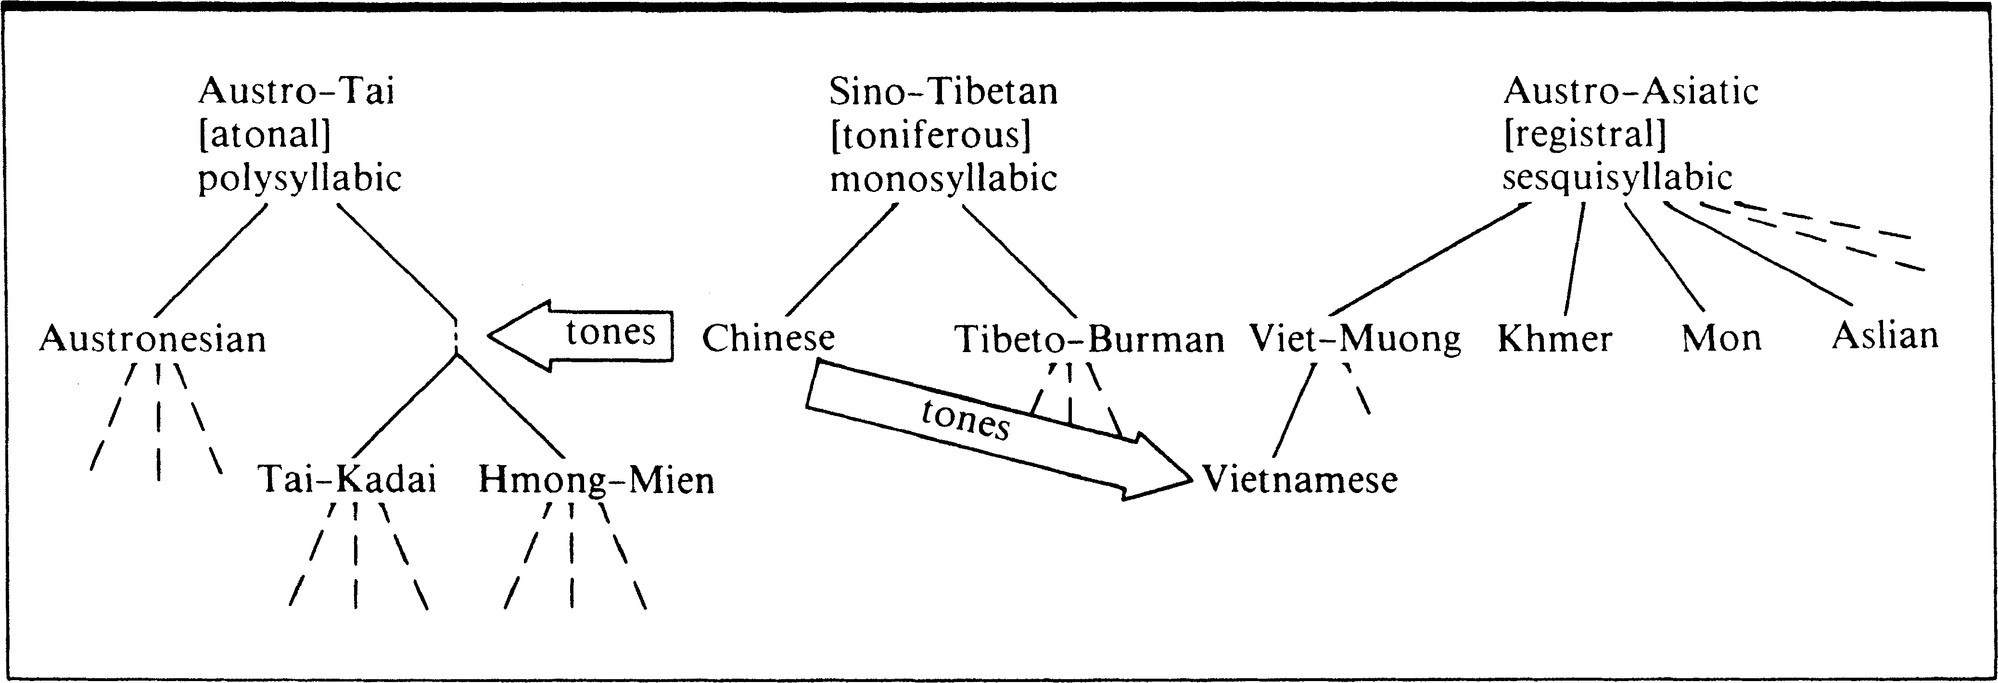
\includegraphics[width=0.9\textwidth]{pics/image34.png}
\end{center}

Features (and vocabulary) can move across language families!

\end{frame}



\begin{frame}{Summary I}
There are five major linguistic families found in Mainland SEA.

While there are a great number of languages spoken in the region, the
linguistic diversity is 
relatively low, probably due to centuries of language contact and human
population
movement.
\end{frame}


\begin{frame}{Summary II}

MSEA languages are characterized by:

\begin{itemize}
\item isolating word formation\\
\item tone\\
\item absence of inflectional morphology\\
\item classifier systems\\
\item aspectual and mood systems rather than tense systems\\
\item sentence final particles\\
\item rampant zero anaphora\\
\item serial verb constructions
\item re-duplication
\end{itemize}

Although there are many exceptions

\end{frame}



\end{document}
